\documentclass[12pt]{article}
\usepackage{graphicx,import}
\usepackage[svgnames]{xcolor} 
\usepackage{fancyhdr}
\usepackage{subfig}
\usepackage{hyperref}
\usepackage{enumitem}
\usepackage{cite}
\usepackage[many]{tcolorbox}
\usepackage{listings }
\usepackage[a4paper, total={6in, 8in} , bottom = 25mm , top = 25mm, headheight = 1.25cm , includehead,includefoot,heightrounded ]{geometry}
\usepackage{afterpage}
\usepackage{amssymb}
\usepackage{fancyvrb}
\usepackage{pdflscape}
\usepackage{gensymb}
\usepackage{textcomp}
\usepackage{xecolor}
\usepackage{rotating}
\usepackage{pdfpages}
\usepackage[Kashida]{xepersian}
\usepackage[T1]{fontenc}
\usepackage{tikz}
\usepackage[utf8]{inputenc}
\usepackage{PTSerif} 
\usepackage{seqsplit}

\usepackage[edges]{forest}

\usepackage{listings}
\usepackage{xcolor}

\hypersetup{
	colorlinks   = true, %Colours links instead of ugly boxes
	urlcolor     = blue, %Colour for external hyperlinks
	linkcolor    = blue, %Colour of internal links
	citecolor   = red %Colour of citations
}
 
\definecolor{codegreen}{rgb}{0,0.6,0}
\definecolor{codegray}{rgb}{0.5,0.5,0.5}
\definecolor{codepurple}{rgb}{0.58,0,0.82}
\definecolor{backcolour}{rgb}{0.95,0.95,0.92}
 
\NewDocumentCommand{\codeword}{v}{
\texttt{\textcolor{blue}{#1}}
}
\lstset{language=java,keywordstyle={\bfseries \color{blue}}}

\lstdefinestyle{mystyle}{
    backgroundcolor=\color{backcolour},   
    commentstyle=\color{codegreen},
    keywordstyle=\color{magenta},
    numberstyle=\tiny\color{codegray},
    stringstyle=\color{codepurple},
    basicstyle=\ttfamily\normalsize,
    breakatwhitespace=false,         
    breaklines=true,                 
    captionpos=b,                    
    keepspaces=true,                 
    numbers=left,                    
    numbersep=5pt,                  
    showspaces=false,                
    showstringspaces=false,
    showtabs=false,                  
    tabsize=2
}

\lstset{style=mystyle}

\settextfont[Scale=1.2 ,BoldFont={Bahij Nazanin-Bold.ttf} , ItalicFont = {IRNazaninIranic.ttf}]{Bahij Nazanin-Regular.ttf}
\setlatintextfont[Scale = 1.0]{Garamond}
\DefaultMathsDigits 
\DeclareMathSizes{11}{19}{13}{9} 
%\DeclareMathSizes{12}{14.4}{8}{9}





\newenvironment{changemargin}[2]{%
\begin{list}{}{%
\setlength{\topsep}{0pt}%
\setlength{\leftmargin}{#1}%
\setlength{\rightmargin}{#2}%
\setlength{\listparindent}{\parindent}%
\setlength{\itemindent}{\parindent}%
\setlength{\parsep}{\parskip}%
}%
\item[]}{\end{list}}


\definecolor{foldercolor}{RGB}{124,166,198}

\tikzset{pics/folder/.style={code={%
    \node[inner sep=0pt, minimum size=#1](-foldericon){};
    \node[folder style, inner sep=0pt, minimum width=0.3*#1, minimum height=0.6*#1, above right, xshift=0.05*#1] at (-foldericon.west){};
    \node[folder style, inner sep=0pt, minimum size=#1] at (-foldericon.center){};}
    },
    pics/folder/.default={20pt},
    folder style/.style={draw=foldercolor!80!black,top color=foldercolor!40,bottom color=foldercolor}
}

\forestset{is file/.style={edge path'/.expanded={%
        ([xshift=\forestregister{folder indent}]!u.parent anchor) |- (.child anchor)},
        inner sep=1pt},
    this folder size/.style={edge path'/.expanded={%
        ([xshift=\forestregister{folder indent}]!u.parent anchor) |- (.child anchor) pic[solid]{folder=#1}}, inner xsep=0.6*#1},
    folder tree indent/.style={before computing xy={l=#1}},
    folder icons/.style={folder, this folder size=#1, folder tree indent=3*#1},
    folder icons/.default={12pt},
}

\begin{document}


%%% title pages
\begin{titlepage}
\begin{center}
        
\vspace*{0.7cm}


\includegraphics[width=0.4\textwidth]{sharif1.png}\\
\vspace{0.5cm}
\textbf{ \Huge{\emph ‌اندازه‌گیری و کنترل کامپیوتری} }\\
\vspace{0.5cm}
\textbf{ \Large{ تمرین ششم} }
\vspace{0.2cm}
       
 
      \large \textbf{دانشکده مهندسی کامپیوتر}\\\vspace{0.2cm}
    \large   دانشگاه صنعتی شریف\\\vspace{0.2cm}
       \large   ﻧﯿﻢ سال دوم 00-99 \\\vspace{0.2cm}
      \noindent\rule[1ex]{\linewidth}{1pt}
استاد:\\
    \textbf{{جناب آقای دکتر همت‌یار}}


    \vspace{0.15cm}
نام و نام خانوادگی:\\

       
    \textbf{{امیرمهدی نامجو - 97107212}}
\end{center}
\end{titlepage}
%%% title pages


%%% header of pages
\newpage
\pagestyle{fancy}
\fancyhf{}
\fancyfoot{}
\cfoot{\thepage}
\chead{تمرین ششم}
\rhead{
\includegraphics[width=0.1\textwidth]{sharif.png}}
\lhead{امیرمهدی نامجو}
%%% header of pages

\KashidaOff


\section*{سوال 2}
$$\lambda f = c$$

$$\lambda = (3 \times 10^8) / (6.5 \times 10^{14}) = 4.62 \times 10^{-7} = 462 nm = 4620 \text{\AA}$$

\section*{سوال 4}

$$R = r + d \tan(\theta)$$
$$R = 0.02 + 60 \tan(1.2 \deg)$$
$$R = 1.277 m$$

در نتیجه اندازه پرتو در 60 متری معادل دایره ای با شعاع $1.277$ متر است.
$$I = P/A \rightarrow = \frac{100 mW} {\pi (1.277)^2 m^2} = \frac{0.1}{5.123} = 0.0195 W/m^2 = 0.00195 mW/cm^2$$

\section*{سوال 6}

یک کاندلا توانی معادل
 $\frac{1}{683}$
  را بر سطحی در فاصله $R$ که مساحت $R^2$ دارد اعمال می کند. با توجه به این موضوع، اگر کره ای به شعاع $R$ را حول منبع به مرکزیت آن در نظر بگیریم، در نظر بگیریم که مساحت
   $4\pi R^2$
دارد، داریم:
$$P = I A = \frac{\frac{1}{683}}{R^2}(4\pi R^2) = 0.0183988 W$$

\section*{سوال 8}

$$E_{photon} = \frac{hc}{\lambda} = \frac{6.62607015\times10^{-34} \times 299792458}{700 \times 10^{-9}} = 2.83778\times10^{-19}$$

$$I = P/A = \frac{P}{\pi D^4/4} = \frac{2\times 10^{-4}}{\pi (5\times 10^{-2})^2/4} = 0.102 W/m^2$$

$$P_d = I \times A = 0.102 \times (\pi \times (2\times 10^{-3})^2/4) =3.2044 \times 10^{-7}$$

$$N  = P_d / E_{photon} = \frac{3.2044 \times 10^{-7}}{2.83778\times10^{-19}} = 1.129 \times 10^{12} \frac{{photons}}{s} $$


\section*{سوال 10}

برای حل این سوال عملا باید بخشی از سوال 9 را هم حل کنیم. طبق نمادگذاری کتاب، بخش مربوط به مسئله قبل را با 2 نماد گذاری می کنیم.

$$R_{2}(t) = R_i + (R_f - R_i)(1 - e^{t/\tau})$$

$$R_2(20ms) = 150 +(45-150)[1-e^{-20/73}] = 124.8k\Omega$$

$$R_1(20ms) = 150 +(85-150)[1-e^{-20/73}] = 134.4 k\Omega$$

همچنین می دانیم که در حالت تاریکی مقاومت $150k\Omega$ است. برای همین موضوع، فرض می کنیم که این سلول در یک سیستم تقسیم ولتاژ با یک مقاومت $150k\Omega$ ای دیگر قرار دارد. در این صورت با فرض $V_s = 5V$ داریم:
$$V_1 =(150 / (134.4 + 150))\times 5 \approx 2.64 V$$
$$V_2 = (150/(124.8+150))5 = 2.73$$

در نتیجه این ولتاژهای مرجع مقایسه گر باید باشند. برای ولتاژ Clear هم حدود $2.51V$ را در نظر می گیریم و همه را در یک مدار تقسیم مقاومتی بزرگتر قرار می دهیم.

فرض می کنیم که در پایین شکل درست قبل از یک مقاومت $1k\Omega$ ای که به زمین وصل است، ولتاژ $2.51v$ تشکیل شود.

در این صورت برای تشکیل ولتاژ $2.64$ و بدست آوردن مقاومت مربوطه داریم:

$$2.51 + R \times (2.51/1000) = 2.64 \rightarrow R=51.79 \Omega$$

برای تشکیل ولتاژ $2.73$ هم داریم:

$$2.67 + R \times(2.51/1000) =2.73 \rightarrow R= 23.9 \Omega$$

برای مقاومت آخری که باید به $5$ ولت ختم شود هم داریم:

$$2.73 + R \times (2.51/1000) = 5 \rightarrow R = 904 \Omega$$

در شکل زیر یک پالس Generator به صورت One-Shot گذاشته شده است که یک پالس یک میلی ثانیه ای برای Clear مدار تولید کند.

سیگنال مربوط به قرمز در صورتی تولید می شود که فلیپ فلاپ مربوط به حالت سبز حالت $0$ را بگیرد. بدین ترتیب می فهمیم که ولتاژ به $2.64$ رسیده ولی به $2.73$ نرسیده است. به همین دلیل برای رعایت این شرایط یک گیت NOT هم گذاشته شده است. توجه کنید که حالت سبز عملا یعنی ولتاژ بالای $2.73$ که یعنی هر دو شرایط ایجاد شده باشد و در نتیجه هر دو باید $1$ باشند. شکل نهایی در صفحه بعد قرار دارد.


\begin{center}
	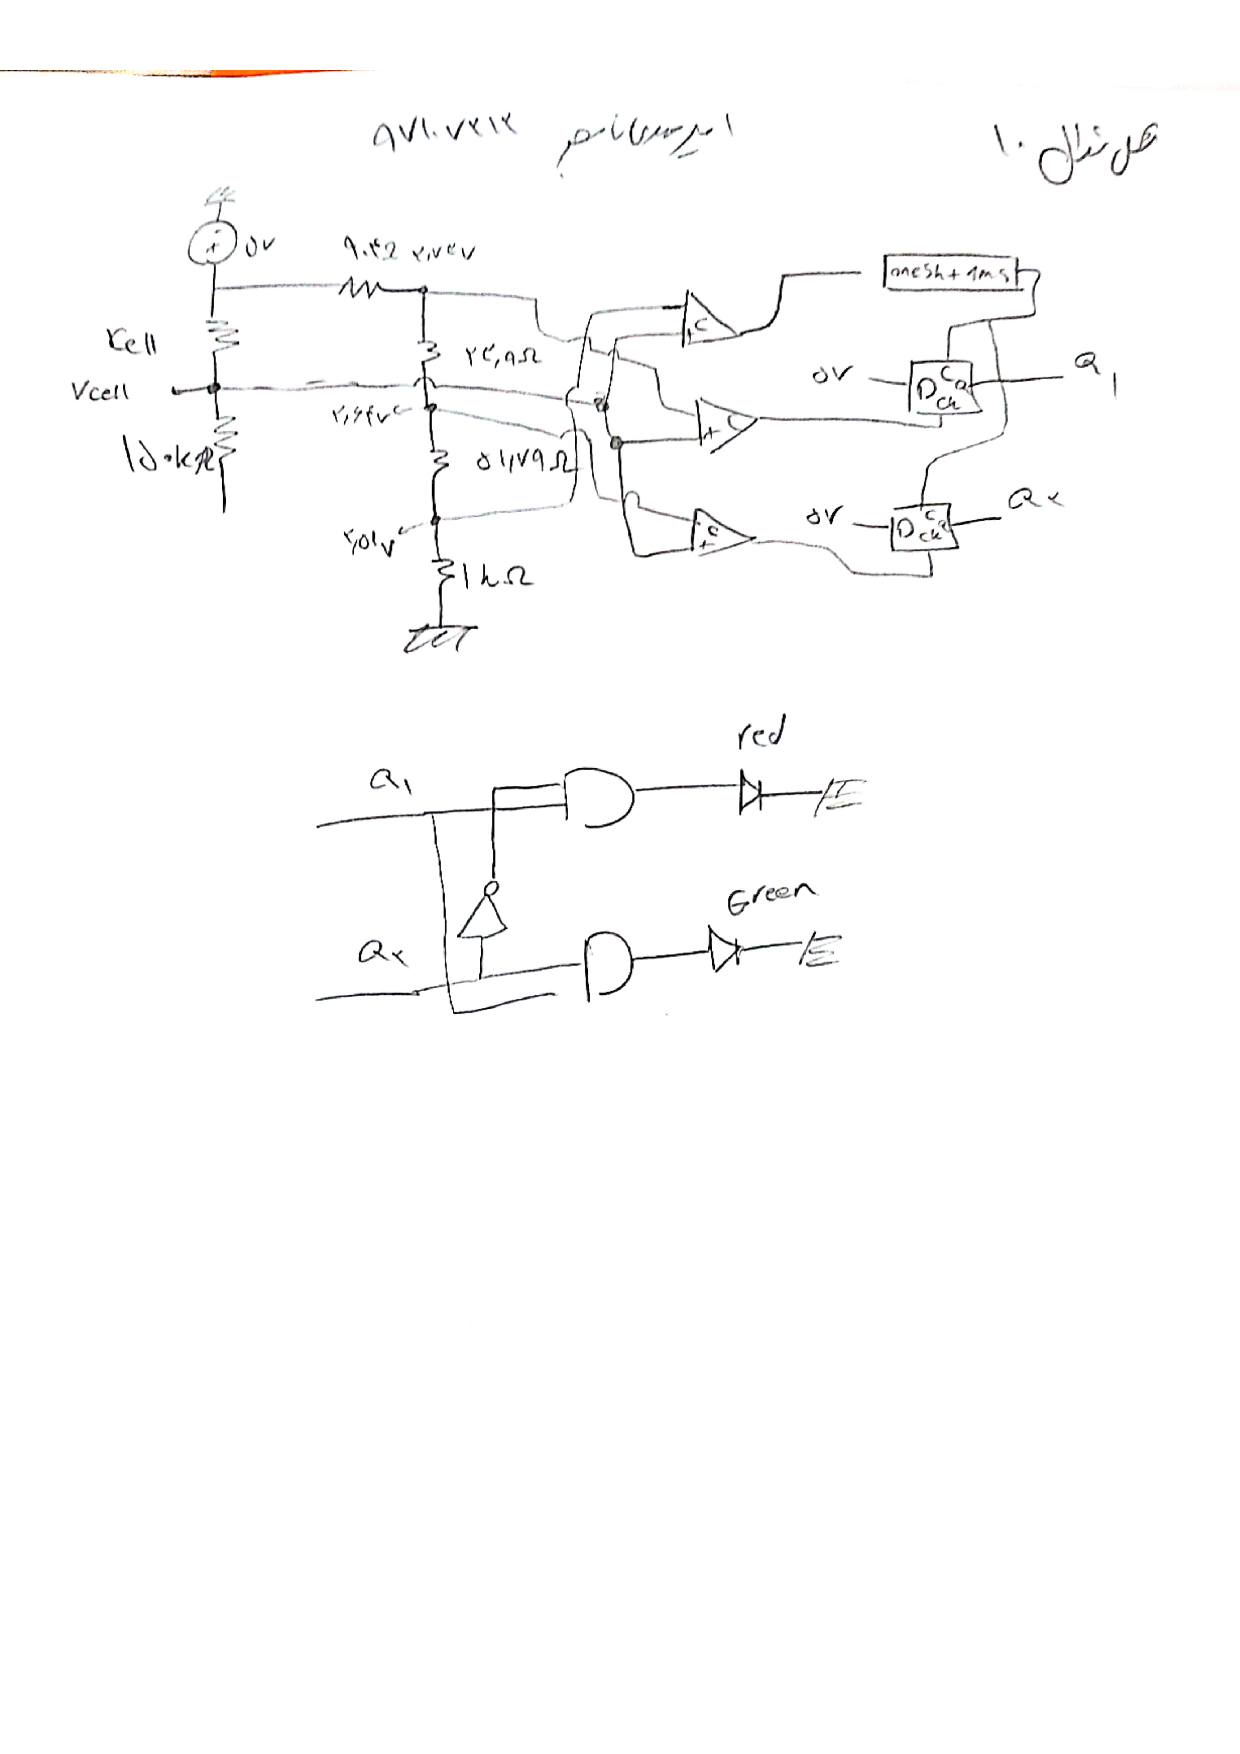
\includegraphics[width = 1.0 \textwidth]{images/10.pdf}
\end{center}
\newpage
\section*{سوال 12}

طبق شکل کتاب مقاومت در $20mW/cm^2$ برابر $2.9k\Omega$ و مقاومت در
$100mW/cm^2$
برابر
$0.5k\Omega$
است. در نتیجه با تشکیل دستگاه دو معادله دو مجهول داریم:
$$1 = m(0.5k\Omega) + V_0$$
$$0.2 = m (2.9 k\Omega) + V_0$$

از این جا داریم:

$$m =\frac{-1}{3} V/k\Omega , V_0 = \frac{7}{6} V$$

شکل را با ترکیب یک \lr{Inverting Amplifier} و یک \lr{Summing Amplifier} رسم می‌کنیم.



\begin{center}
	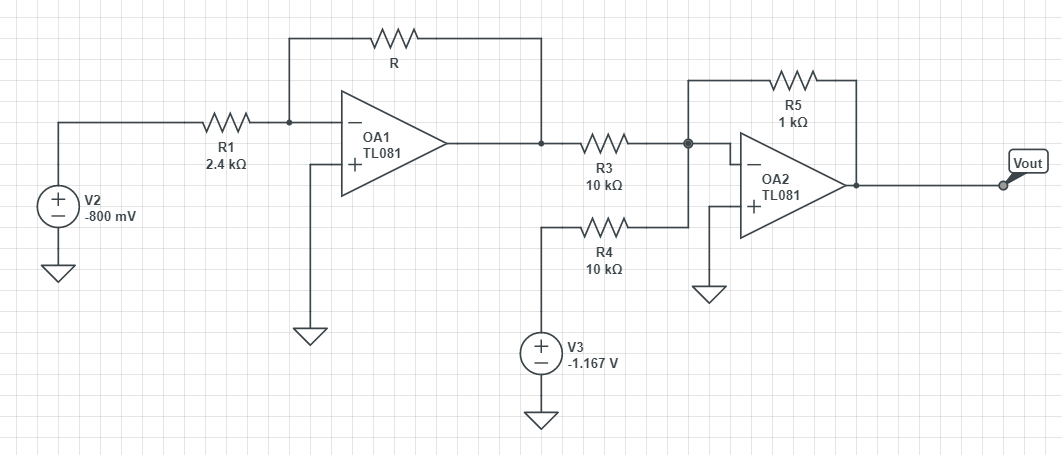
\includegraphics[width = 1.0 \textwidth]{images/12.png}
\end{center}

\newpage
\section*{سوال 14}

ابتدا مقاومت مدار نهایی را بدست می آوریم:

$$R_f = V_{f}^{2} / P = 81/0.5 = 162 \omega$$

مقاومت یک سلول هم با توجه به رابطه داده شده برای ولتاژ مدار باز و جریان مدار بسته بدست می‌آید:

$$R=\frac{0.6}{0.015}=40$$

فرض می کنیم آرایش ما به این صورت باشد که $n$ ستون موازی داشته باشیم که هر کدام از $m$ سلول سری تشکیل شده است و در نهایت همه این‌ها به یک خروجی
 $R_f$
  متصل هستند.
ولتاژ دو سر چنین مداری برابر $m V$‌ و مقاوت معادل آن به صورت موازی $n$ عدد مقاومت $mR$ است یعنی
$R_{thevenin} = \frac{mR}{n}$

در اصل چنین مداری اگر معادل یک مدار تونن بشود، بهتر است که مجموعه کل مقاومت‌های آن در کنار مقاومت $R_f$  دیگر برابر $2R_f$ بشود. یعنی مقاومت مجموعه کل سلول‌ها بدون مقاومت اصلی بیرونی مدار باید برابر $R_f$ بشود. همچنین با توجه به این که در مدا نهایی عملا $2R_f$ مقاومت داریم، باید ولتاژ تولیدی هم دوبرابر ولتاژ کلی خواسته شده در سوال باشد.

$mV_{cell} = 2 V_f \rightarrow \times 0.6 = 18 \rightarrow m = 30$
و
$mR/n = R_f \rightarrow \frac{30 \times 40}{n} = 162 \rightarrow n=7.4 \rightarrow n=8$ 

مدار نهایی به این شکل است: (شکل قابل زوم کردن است)


\begin{center}
	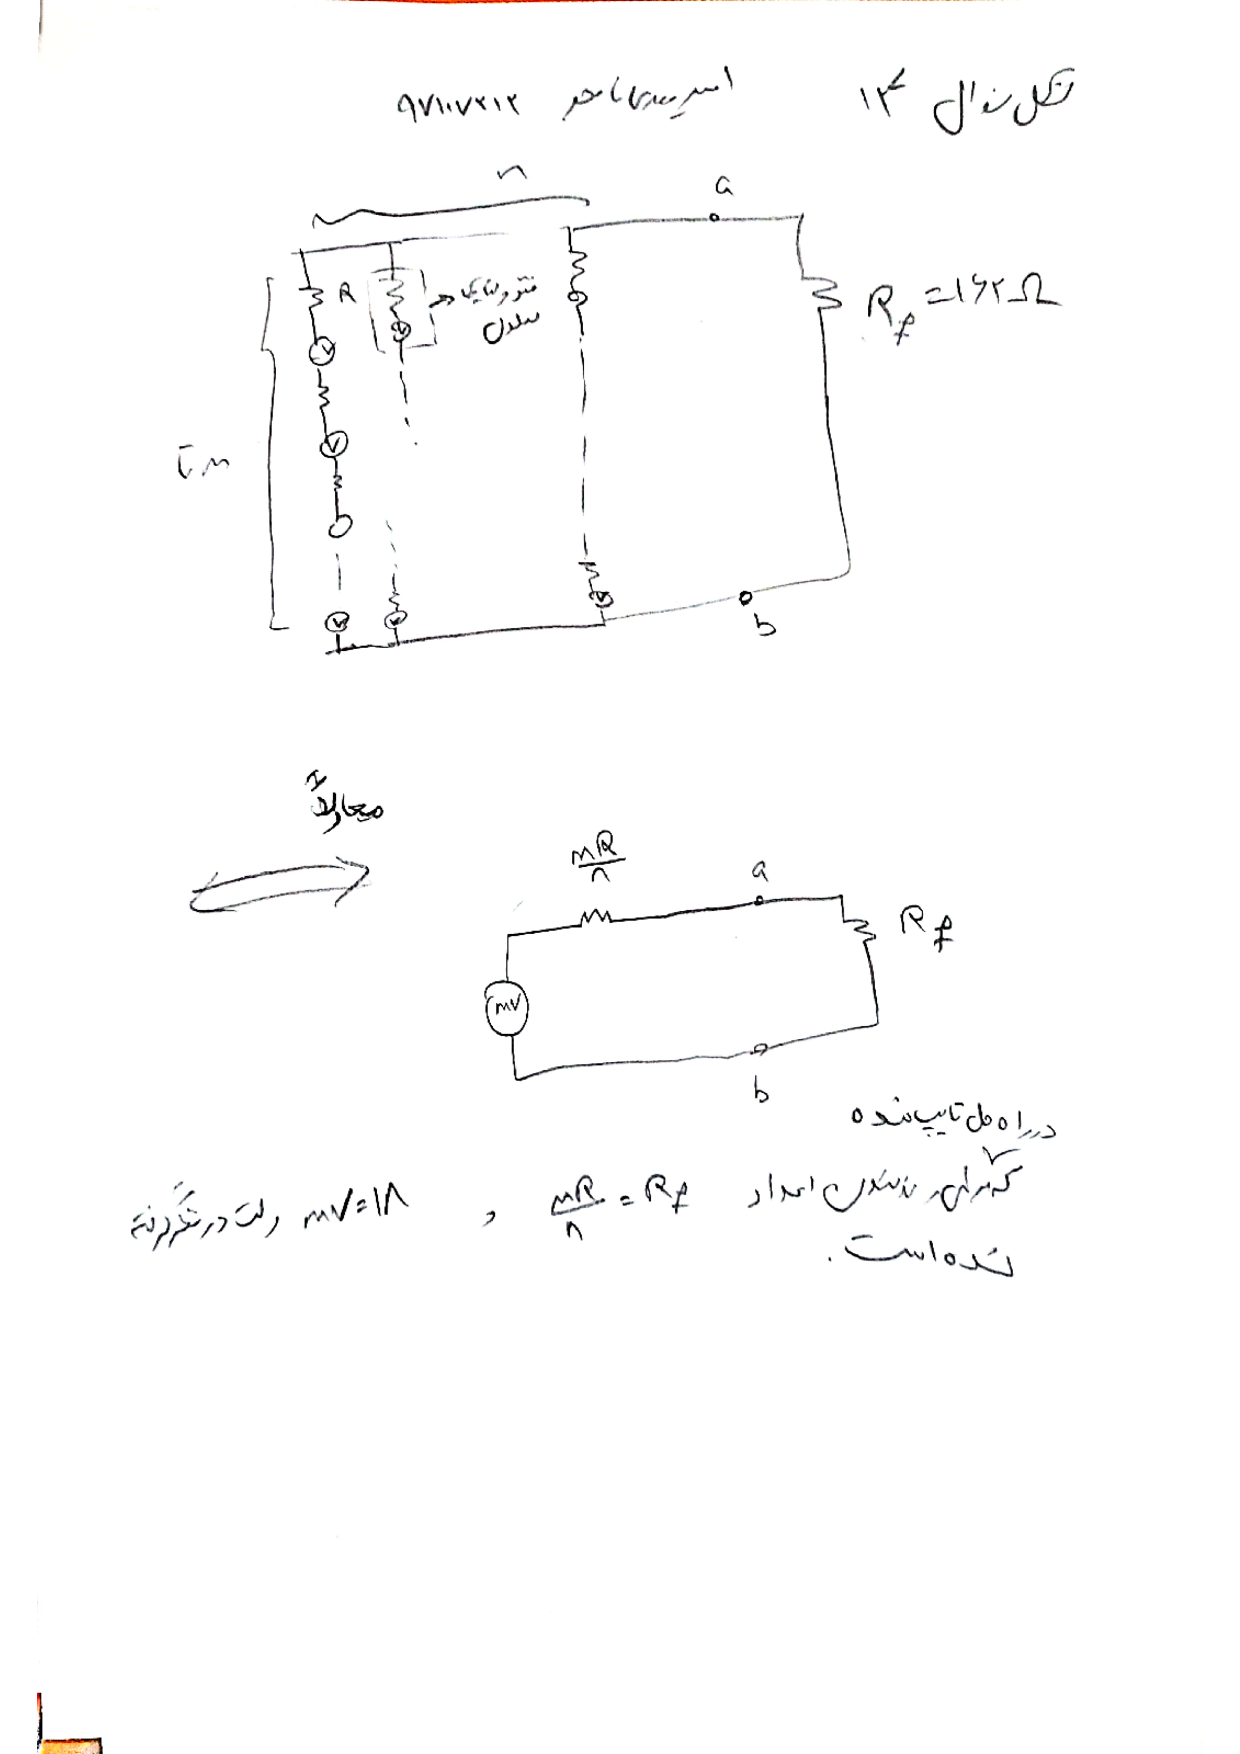
\includegraphics[width = 0.4 \textwidth]{images/12.pdf}
\end{center}
\newpage

\section*{سوال 16}



باید دو مقاومت $10$ و $100$ اهمی را موازی بگیری مک ه بتوانیم روابط مربوط به جریان و ولتاژ را بدست بیاوریم. این دو مقاومت موازی باعث مقاومت معادل $9.09$ می‌شوند. در نتیجه

$$420 I_c + v_{ce} + 9.09 I_c = 10$$

وقتی که $I_c=0$ است داریم
 $V_{ce} =10V$ و وقتی
$V_{ce} = 0$
داریم $I_c = 23.3mA$

یعنی عملا در نمودار داده شده در کتاب باید خطی بکشیم که $23.3$ محور عمودی را به $10$ محور افقی وصل کرده و نقاط برخورد آن را ببینیم تا به ازای شدت‌های مختلف جریان را بدست آوریم:


\begin{center}
	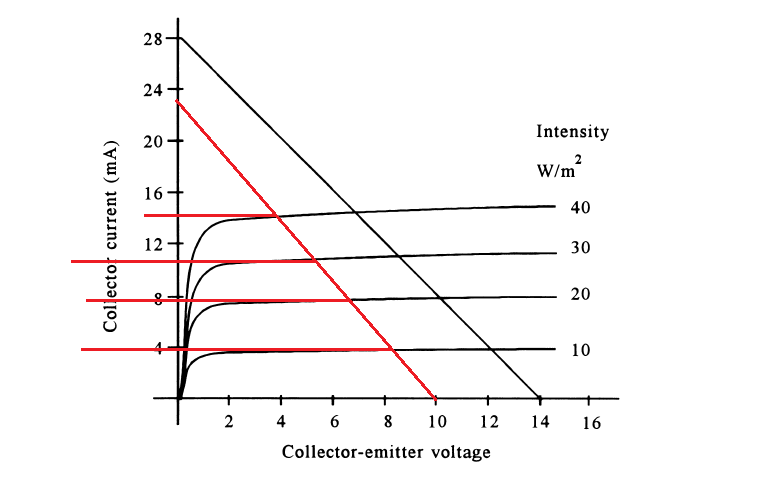
\includegraphics[width = 0.5 \textwidth]{images/16.png}
\end{center}

همچنین توجه داریم که در اصل $10/110$ جریان به مقاومت $100$ اهمی می‌رود و سپس از جریان فیدبک واردخروجی می‌شود. در نتیجه
$$V_{out} = -500 (10/110) I_c = -45.45 I_c$$


 $$
 \begin{array}{|l|l|l|}
 	\hline \text { Intensity }\left(\mathrm{W} / \mathrm{m}^{2}\right) & \text { Collector current }(\mathrm{mA}) & \text { Output voltage (volts) } \\
 	\hline 10 & 4 & -0.18 \\
 	\hline 20 & 7.9 & -0.36 \\
 	\hline 30 & 10.5 & -0.47 \\
 	\hline 40 & 14 & -0.64 \\
 	\hline
 \end{array}
 $$
 
 
 نمودار نهایی به این صورت می‌شود:
 
 
 \begin{center}
 	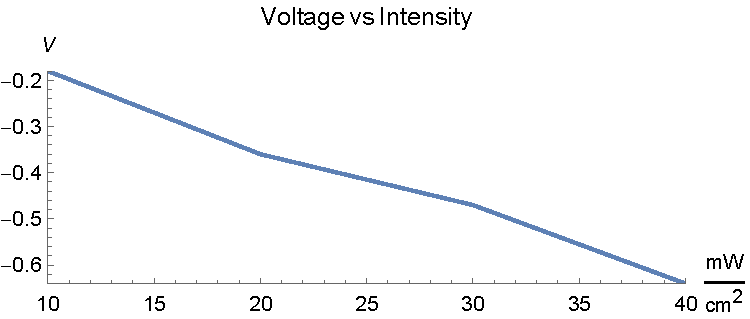
\includegraphics[width = 0.5 \textwidth]{images/16.pdf}
 \end{center}
 
 
 \newpage
 \section*{سوال 18}
 
 $$I = (3\times 10^6)\times(50)\times(1.6\times10^{-19}) =2.4 \times 10^{-11}$$
 
 $$R = V/I \rightarrow R = \frac{3\times 10^{-6}}{2.4\times10^{-11}}$$
 
 $$R=125 k\Omega$$
 
  \section*{سوال 20}
  
  چنین سیستمی را در نظر می‌گیریم. 
   \begin{center}
  	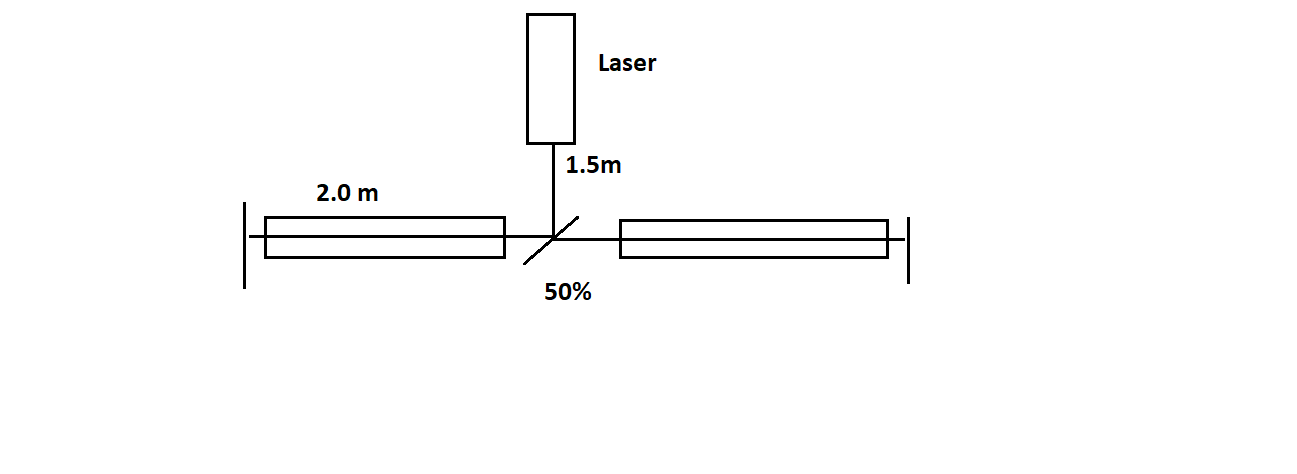
\includegraphics[width = 0.5 \textwidth]{images/20.png}
  \end{center}
  
  پرتو عملا باید مسافت $3.5$ متری را بپیماید. پس شعاع آن در هنگام رسیدن به آشکارساز برابر خواهد بود با:
  
  $$R = r + l \tan(\theta) = 1 \times 10^{-3} + 3.5 \tan(2.2\times 10^{-3}) = 0.0087$$
  
  مساحت پرتو در این نقطه برابر است با
  
  $$A = \pi R^2 = \pi (0.0087)^2 = 0.0002377$$
  
  همچنین توانی پرتو یک بار در اثر تقسیم شدن نصف می‌شود و سپس به ازای هر متر $12\%$ کاهش می‌یابد. یعنی ابتدا توان $2.1mW/2 = 1.05mW$ شده و سپس $24\%$ کاهش یافته و برابر خواهد بود با:
  $$(1-0.24) \times 1.05 mW = 0.798 mW$$
  
  در نتیجه شدت نور در آشکارگر برابر خواهد بود با:
  
  $$I=\frac{P}{A} = \frac{0.798 \times 10^{-3}}{2.377 \times 10^{-4}} \approx 3.32 W/m^2$$
  
  
    \section*{سوال 22}
  
  ابتدا به شکل داده شده در کتاب توجه کنید:
  
   \begin{center}
  	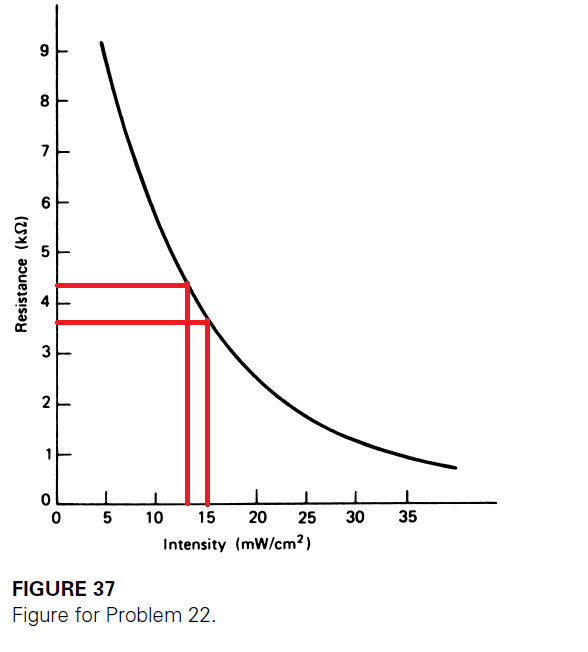
\includegraphics[width = 0.25 \textwidth]{images/22.png}
  \end{center}

طبق این شکل به ازای $15mW/cm^2$ مقاومت $3.6k\Omega$ و به ازای $10$ درصد کمتر از آن یعنی $13.5mW/cm^2$ مقاومت $4.4k\Omega$ است.

با فرض منبع تغذیه $10$ ولتی مسئله را حل می‌کنیم.

اگر از این خاصیت مقاومتی در یک مدار تقسیم ولتاژ استفاده کنیم و این مقاومت در قسمت متصل به زمین باشد و مقاومت دیگر هم $10k\Omega$ باشد، ولتاژ در حالت $3.6k\Omega$ به صورت زیر است:

$$V_{3.6k\Omega} = 10 \times \frac{3.6}{3.6+10} = 2.647 V$$

 به ازای مقاومت $4.4k\Omega$ مقدار ولتاژ برابر خواهد بود با
 $$V_{4.4k\Omega} = 10 \times \frac{4.4}{10+4.4} = 3.056V$$
 
 در حالت اول ولتاژ نظیر به هر دو سلول برابر خواهد بود و اختلاف ولتاژ نهایی آنان صفر می شود. اما در حالت دوم این اختلاف ولتاژ برابر
 $\Delta V = 3.056 - 2.647 = 0.409V$
 می شود. با فرض این که بخواهیم زنگ هشدار را با ولتاژ $5V$ تنظیم کنیم، نیاز به تقویت اختلاف ولتاژ بالا با بهره
 $\frac{5}{0.409}=12.225$
 خواهیم داشت. در نتیجه از یک  \lr{Differential Amplifier} 
 استفاده می‌کنیم که هم عمل تفاضل را انجام داده و هم تقویت مد نظر را انجام بدهیم. برای ایجاد ولتاژ $5$ ولت هم از یک مدار تقسیم ولتاژ برابر ساده استفاده می‌کنیم. نتیجه نهایی به صورت شکل زیر خواهد بود:
 
   
 \begin{center}
 	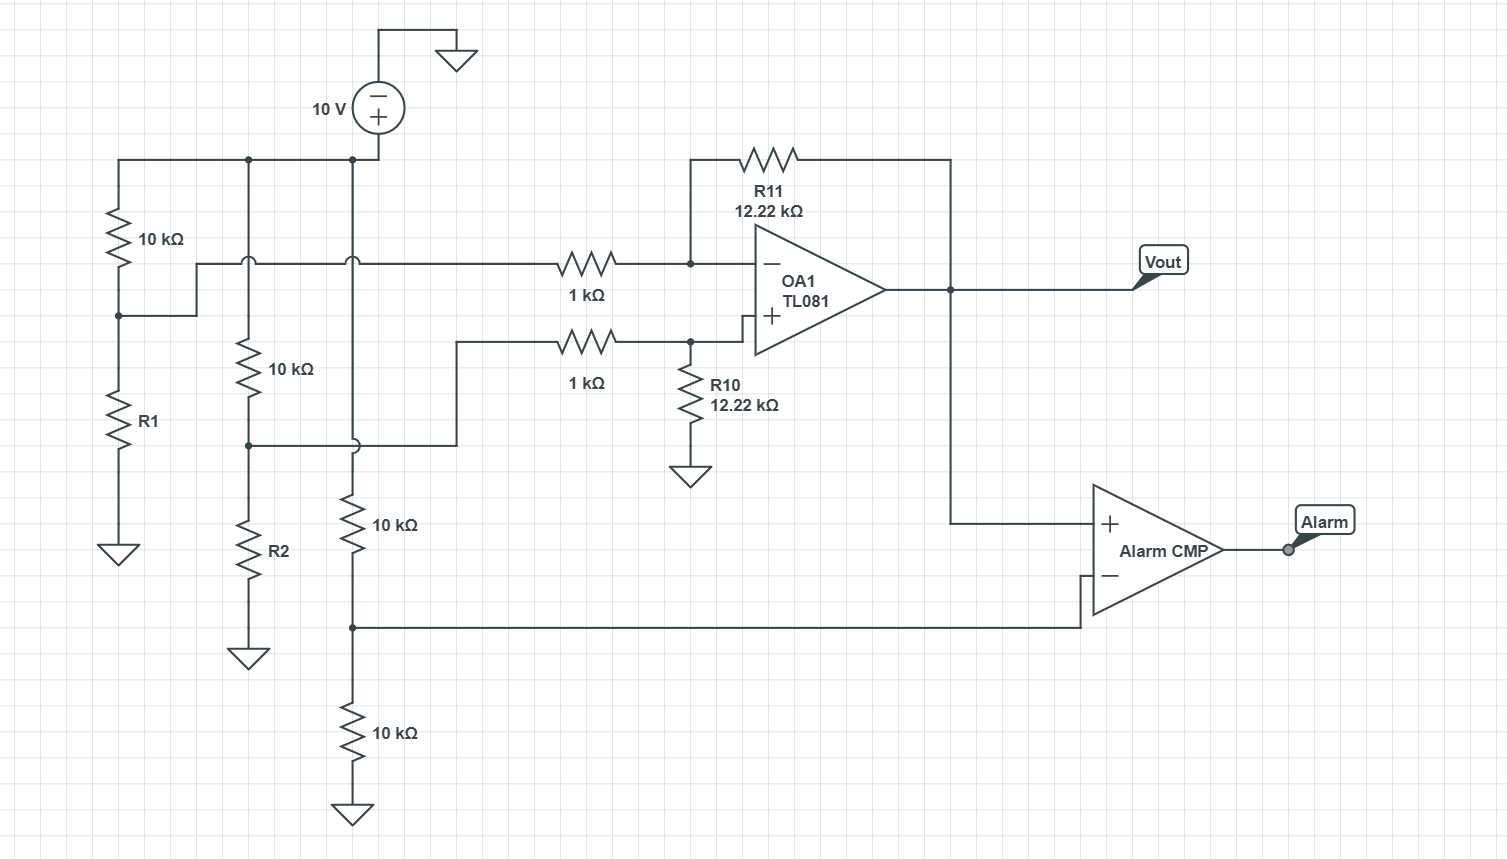
\includegraphics[width = 0.5 \textwidth]{images/22-2.png}
 \end{center}
 
 
\end{document}



